\documentclass[debug,nodate,hideweeklyreports]{polytech/polytech}
      
\usepackage{lipsum}
\usepackage{listings}
\usepackage{biblatex}
\usepackage{float}
\usepackage{hyperref}
  
\typereport{prddi5}
\schooldepartment{di}

\reportyear{2018-2019}

\title{Détecteur multi-objets dans des images naturelles exploitant un graphe de relations spatiales}

\student{Julien}{Cheny}{julien.cheny@etu.univ-tours.fr}

\academicsupervisor[di]{Jean-Yves}{Ramel}{jean-yves.ramel@univ-tours.fr}

\resume{
}
\abstract{
}
\motcle{mot}
\keyword{word}

\posterblock{Contexte}
{
    La détection multi objet dans une image numérique est un incontournable de la reconnaissance de formes et de l’analyse d’images. 
    
    
    Cette méthode est exploitable dans de nombreux domaines.
    Nous pouvons citer le secteur de la santé, surveillance, automobile, robotique, etc.
}
{images/T_sampledetect.png}
{Exemples de détections d'objets}

\posterblock{Objectifs}
{
    Améliorer le détecteur d’objets YOLO en utilisant un graphe de relations spatiales.
    
    
    Connaître les objets qui pourraient potentiellement apparaître à côté d'un objet déjà identifié afin de mieux les détecter.
}
{images/H_structgen2use.png}
{Structure du système}

\posterblock{Réalisations}
{
    \begin{itemize}
    \item Générateur de graphe de relations spatiales
    \item Générateur de paramètres d'apprentissage pour détecteur d'objets
    \item Multiple détecteur successif utilisant le graphe de relations spatiales
    
    \end{itemize}
}
{images/S_graphe80class.png}
{Graphe de relations spatiales généré}

\newglossaryentry{framework}
{
	name=Framework,
	description={Ensemble d'outils et de composants logiciels organisés conformément à un plan d'architecture et des patterns}
}

\newglossaryentry{opensource}
{
	name=Open Source,
	description={Libre de droits, dont les codes sources sont disponibles et modifiables librement}
}

\newglossaryentry{machinelearning}
{
	name=Machine learning,
	description={Champ d'étude de l'intelligence artificielle qui se base sur des approches statistiques pour donner aux ordinateurs la capacité d'apprendre à partir de données, c'est-à-dire d'améliorer leurs performances à résoudre des tâches sans être explicitement programmés pour chacune}
}

\newglossaryentry{deeplearning}
{
	name=Deep learning,
	description={Ensemble de méthodes d'apprentissage automatique tentant de modéliser avec un haut niveau d’abstraction des données grâce à des architectures articulées de différentes transformations non linéaires}
}

\newglossaryentry{gnu}
{
	name=GNU,
	description={système d’exploitation libre. Il reprend les concepts et le fonctionnement d’UNIX}
}
\newglossaryentry{cuda}
{
	name=CUDA,
	description={technologie de \gls{gpgpu}, c'est-à-dire utilisant un processeur graphique (GPU) pour exécuter des calculs généraux à la place du processeur (CPU)}
}

\newacronym{api}{API}{Application Programming Interface}
\newacronym{irm}{IRM}{Imagerie par Résonance Magnétique}
\newacronym{cnn}{CNN}{Réseau Neuronal Convolutif}
\newacronym{uml}{UML}{Unified Modeling Language}
\newacronym{nms}{NMS}{Non-Maximum Suppression}
\newacronym{svm}{SVM}{Support Vector Machine}
\newacronym{rpn}{RPN}{Region Proposal Network}
\newacronym{gpgpu}{GPGPU}{General-Purpose Computing on Graphics Processing Units}
\newacronym{cudnn}{cuDNN}{NVIDIA CUDA Deep Neural Network}

\bibliography{biblio}

\makeglossaries

\begin{document}
             
\chapter{Introduction}

Dans ce document, nous allons aborder l’ensemble des spécifications et la planification du Projet de Recherche et Développement « Détecteur multi-objets dans des images naturelles exploitant un graphe de relations spatiales ». Ce projet a été réalisé dans le cadre de la dernière année du cycle d’ingénieur informatique à Polytech Tours. 
Ce projet a été proposé par M. Jean Yves RAMEL qui en est l’encadrant. Le développement est soutenu par M. Gaëtan GALISOT afin d’apporter des connaissances supplémentaires au sujet. Julien CHENY est l’étudiant assimilé maîtrise d’œuvre et auteur de ce document. Enfin, la réalisation du cahier des spécifications est supervisée par M. Nicolas RAGOT.

\section{Contexte de la réalisation}

La détection multi-objets dans une image numérique est un incontournable de la reconnaissance de formes et de l’analyse d’images. 
Cette méthode est exploitable dans de nombreux domaines.
Nous pouvons citer le secteur de la santé avec le traitement d’image médicale. Ces traitements sont appliqués à des \gls{irm} afin de détecter des changements ou des anomalies.
Le secteur de la surveillance et sécurité est aussi touché par cette méthode avec la reconnaissance faciale. Ce système vise à reconnaître une personne grâce à son visage afin d’actionner une alerte ou un déverrouillage. La reconnaissance faciale est aussi utilisée sur certains réseaux sociaux dans le but de faciliter la vie aux utilisateurs en identifiant automatiquement les personnes sur une image postée.
En automobile, de nombreux projets sont réalisés dans le but de supprimer l’intervention du conducteur et ainsi rendre le véhicule autonome. Ce système devrait réduire fortement les risques d’accident. Des enquêtes scientifiques menées en France entre 1983 et 2004 ont montré que dans 90 \% des accidents mortels le comportement humain est en jeu.
Aussi, le secteur de la robotique est évidemment impliqué dans la recherche sur cette méthode puisqu’elle permet de simuler des fonctions du cerveau humain en s’en inspirant fortement.
Nous pouvons citer de manière plus généraliste la recherche d’image par contenu ou par mots-clés, technique permettant de rechercher des images à partir de ses caractéristiques visuelles. Cette technique est utilisée par Google Image en vue de donner plus de paramètres de recherche à l’utilisateur.
Pour résumé, cette méthode peut être appliquée au secteur de la santé, surveillance, automobile, robotique, etc. Les possibilités sont nombreuses et permettraient le remplacement de taches humaines, impliquant des ressources conséquentes. 
En utilisant des concepts en plein essor de \gls{machinelearning}, cela en fait une cible récurrente à la recherche d’améliorations.

\section{Objectifs}

L’intention finale de ce projet consiste à améliorer la détection d’objets par un détecteur choisi. Ce projet a le détecteur d’objets pour seul existant. 
L’axe d’amélioration abordé est l’utilisation d’un graphe de relations spatiales pour redonder une détection plus précise.
Le système se présente sous forme de conteneur logiciel comprenant le détecteur d’objets, le générateur de graphe de relations spatiales et le système permettant la redondance de détection d’objets par l’utilisation de ce graphe.
Ce projet n’a aucune contrainte d’ergonomies ou de simplifications d’utilisation et n’a donc pas d’interface homme-machine.
L’outil de conteneurisation utilisé pour exécuter le système est Docker. En effet, les besoins en termes de ressources matérielles étant très grands, l’aspect portable du système est important pour faciliter le déploiement sur une autre machine ou sur un Cloud.

\section{Hypothèses}

La mise en œuvre d’un détecteur d’objets est parfois non concluante et la durée de résolution des erreurs étant trop longue par rapport au format du projet. Il serait nécessaire, dans ce cas, de changer de détecteur d’objets.
L’apprentissage d’objets au détecteur d’objets nécessite des ressources matérielles conséquentes pendant une durée chiffrée en dizaines d’heures, ou même en jours. Dans le cas où la durée d’apprentissage sur une machine standard dépasse le cadre du projet, plusieurs solutions sont envisageables. Il est possible de passer à une machine (ou instance cloud) plus adaptée à cette utilisation ou diminuer la taille de la base d’images en enlevant des images ou des classes complètes.

\section{Bases méthodologiques}

Pour gérer le développement du projet, nous utilisons GitHub. Ce service permet de versionner le code, ouvrir des issues (problèmes), écrire des wikis et rendre le projet \gls{opensource}.

La collection de documents à rendre est rédigée sous Latex. Les diagrammes de modélisation du système sont réalisés avec le langage \gls{uml}. La planification des taches est quant à elle réalisée avec un diagramme de Gantt. Nous utiliserons la méthode agile pour répondre aux problématiques de pilotage et réalisation du projet. 

\chapter{Description générale}

\section{Environnement du projet}

Le projet n’a pas d’existant semblable, l’utilisation d’un graphe de relations spatiales pour améliorer la détection rend le projet unique. Nous utiliserons cependant un détecteur d’objets existant pour la fonctionnalité « détection d’objets ». 

\begin{figure}[H]
  \pgfimage[width=10cm]{images/A_envirproj.png}
  \caption{Schéma de l'environnement du projet}
  \label{fig:envirproj}
\end{figure}

Pour exécuter le projet, l’utilisateur lance le programme depuis sa machine. Celui-ci récupère des informations d’une base d’images mise à disposition localement à la machine. Ces images sont nécessaires à l’apprentissage du détecteur d’objets. Ensuite, le programme fonctionne localement à la machine afin de répondre aux attentes de l’utilisateur. 

\section{Caractéristiques des utilisateurs}

Nous avons défini un seul utilisateur pour ce projet. En effet, seul un informaticien va être amené à utiliser ce système.

\subsection{Informaticien}

Ce projet vise à être exploité ensuite par d’autres informaticiens rattachés au domaine de la reconnaissance des formes et analyse d’images. Ces utilisateurs pourront déployer la solution et l’exécuter en utilisant le terminal de commandes.
L’informaticien aura un accès complet au système et pourra le modifier afin de l’adapter à son usage. 
Cet acteur aura cependant deux rôles distincts : il sera utilisateur ou entraîneur du système.
En tant qu’utilisateur, il pourra proposer une image au programme et recevoir la liste d’objets détectée dans celle-ci. Et en tant qu’entraîneur, il pourra proposer une base d’images à apprendre afin de créer les graphes de relations spatiales et entraîner les détecteurs d’objets liés à ces graphes.

\section{Fonctionnalités du système}

Avant de pouvoir utiliser le système, il est nécessaire d’effectuer un entraînement en amont. Nous pouvons donc distinguer deux parties à ce système.
\begin{figure}[H]
  \pgfimage[width=16cm]{images/B_fonctsys1user.png}
  \caption{Schéma de fonctionnement du mode utilisation}
  \label{fig:schemfonctuser}
\end{figure}

Dans le schéma \autoref{fig:schemfonctuser}, on peut distinguer l’action principale et finale de l’utilisateur. 
Le projet est exécuté par l’intermédiaire d’une commande de terminal depuis la machine hôte. L’application prend une image en paramètre et retourne une liste d’objets avec une probabilité de correspondance et les coordonnées de la boîte contenant l’objet. L’image va passer une première fois à travers le réseau de neurones d’un détecteur d’objets. Le détecteur d’objets va ensuite être pondéré différemment en fonction des résultats de la détection d’objets précédente et des liaisons interobjet dans le graphe de relations spatiales.  L’image étant amputée des boîtes détectées à chaque itération, le système s’arrête lorsqu’il n’y a plus d’objets détectés. 

\begin{figure}[H]
  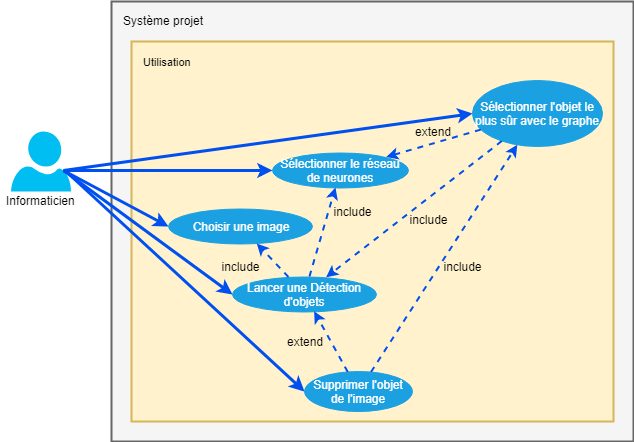
\includegraphics[width=16cm]{images/C_fonctsys2userusecase.png}
  \caption{Diagramme de cas d'utilisation du mode utilisation}
  \label{fig:usecaseuser}
\end{figure}

Dans ce diagramme de cas d’utilisation  \autoref{fig:usecaseuser}, nous pouvons déterminer l’action principale : la détection d’objets. Celle-ci ne peut être effectuée qu’à partir du moment où une image et un réseau de neurones ont été choisis. La sélection du réseau de neurones est ensuite gérée automatiquement après la sélection de l’objet le plus sûr. 

Avant d’utiliser le système, il est impératif de passer par l’étape d’apprentissage.

\begin{figure}[H]
  \pgfimage[width=16cm]{images/D_fonctsys3trainer.png}
  \caption{Schéma de fonctionnement du mode apprentissage}
  \label{fig:schemfonctlearn}
\end{figure}

Le détecteur d’objets fonctionne sur un réseau de neurones, lequel a besoin d’apprendre les objets à détecter grâce à une base d’images. Dans le schéma \autoref{fig:schemfonctlearn}, nous pouvons démontrer le rôle principal et final de l’entraîneur consistant à choisir une base d’images. Celle-ci contenant des images avec de nombreux objets déjà étiquetés. Le système aura ensuite pour but de générer des graphes des relations spatiales interobjet et d’apprendre les réseaux de neurones liés à ces graphes. Chaque classe d’objets apprise a donc son propre graphe où les nœuds représentent des classes d’objets et les arcs correspondent à des histogrammes de probabilité d’orientation de l’objet par rapport à un autre.

\begin{figure}[H]
  \pgfimage[width=16cm]{images/E_fonctsys4graph.png}
  \caption{Exemple de graphe de relations spatiale}
  \label{fig:graphsampl}
\end{figure}

Si nous prenons pour exemple le schéma \autoref{fig:graphsampl}, le graphe correspond à la classe « Humain ». D’après le graphe, un objet « humain » est souvent à côté d’un objet « vélo » ou d’un objet « bus ». En observant l’histogramme de l’arc, entre H et V, nous pouvons remarquer que l’objet « vélo » à 72\% de chance d’être en dessous de l’objet « humain ».
Ce graphe sera utilisé pour générer un réseau de neurones, mais aussi pour intervenir dans le choix du prochain objet sur lequel observer le graphe.

\begin{figure}
  \pgfimage[width=16cm]{images/F_fonctsys5trainerusecase.png}
  \caption{Diagramme de cas d'utilisation du mode apprentissage}
  \label{fig:usecaselearn}
\end{figure}

Dans ce diagramme de cas d’utilisation \autoref{fig:usecaselearn}, nous retrouvons le point central de cette étape : l’apprentissage de différents réseaux de neurones. Celui-ci peut être effectué directement à partir de la base d’images chargées ou après une sélection des objets à apprendre. Cette sélection est réalisée en utilisant le graphe de relations spatiales, généré à partir de la base d’images. De cette étape sont récupérés les poids des réseaux appris et les graphes de relation spatiale.

\section{Structure générale du système}

Le projet dispose d’une structure, elle aussi séparée en deux parties.
La première, toujours liée à l’apprentissage, va nous permettre, en partant d’une base d’images, de récupérer les graphes de relations spatiales interobjet et les réseaux de neurones associés.

\begin{figure}
  \pgfimage[width=16cm]{images/G_structgen1train.png}
  \caption{Schéma de la structure générale du mode apprentissage}
  \label{fig:structlearn}
\end{figure}

Dans ce schéma \autoref{fig:structlearn}, le système suit plusieurs étapes nécessaires à la génération du résultat. 
Tout d’abord, un premier apprentissage du détecteur multi-objets, YOLO, est effectué sur la totalité des objets de la base d’images. Le réseau de neurones et les poids associés à celui-ci vont être enregistrés.
Les autres apprentissages sont effectués en réduisant la base d’images par une sélection d’après les classes d’objets présents dans les graphes.
Par exemple, si le graphe 1 contient les classes bus, humain et vélo, alors les images sélectionnées pour l’apprentissage du réseau associé à ce graphe contiendront des bus, des humains et/ou des vélos. Les autres classes étiquetées dans ces images, comme un oiseau dans une image contenant un vélo, sont ignorées.
Les programmes qui seront créés au sein de ce projet utiliseront le langage Python.

La seconde partie du projet représente l’utilisation du système. Celle-ci a pour but de détecter les objets présents dans l’image qui lui est passée en paramètre.

\begin{figure}
  \pgfimage[width=16cm]{images/H_structgen2use.png}
  \caption{Schéma de la structure générale du mode utilisation}
  \label{fig:structuse}
\end{figure}

Dans ce schéma \autoref{fig:structuse}, YOLO est utilisé en « mode détection » afin de détecter les objets dans l’image. Au début, une première détection est effectuée par un réseau de neurones connaissant tous les objets. De cette détection, résulte une liste d’objets, avec pour chacun d’eux une probabilité de correspondance et la boîte dans laquelle ils se trouvent. Ensuite, le programme Ranking choisit l’objet le plus probable parmi les probabilités de correspondance proposées par YOLO. Cet objet est enregistré puis supprimé de l’image et un nouveau réseau de neurones est appliqué au détecteur multi-objets, celui de l’objet choisi. L’image amputée effectue un second passage dans le détecteur. À partir du second passage, le programme de Ranking utilise le graphe de l’objet détecté au passage précèdent afin d’améliorer le processus de choix. Le système se poursuit jusqu’à ce qu’il n’y ait plus d’objets retournés par le détecteur multi-objets.

\chapter{Etat de l'art/veille}
\section{Le Réseau de neurones artificiel}

Un réseau neuronal artificiel est un paradigme de traitement de l’information inspiré des systèmes nerveux biologiques qui, comme le cerveau, traitent de l’information. L'idée principale de ce système consiste à interconnecter un grand nombre d’éléments de traitement (neurones) ayant pour but de résoudre un problème. Comme nous apprenons de nos expériences, le réseau neuronal apprend grâce à des données. Plus il y a de données apprises, plus le réseau est précis et efficace. Grâce au processus d’apprentissage, les réseaux neuronaux vont permettre la reconnaissance de modèle ou la classification de données. Comme dans les réseaux biologiques on retrouve aussi les synapses dans les réseaux artificiels.

Dans un réseau neuronal artificiel, les neurones sont regroupés dans plusieurs couches. À l’intérieur d’une couche, les neurones ne sont pas connectés entre eux. Cependant, entre deux couches, les neurones sont complètement connectés. On peut distinguer trois types de couches. La couche d’entrée (input layer) va accueillir les informations à apprendre, classifier ou traiter. Les couches cachées (hidden layer) vont transformer la couche d’entrée en différents états de transition. La couche de sortie (output layer) contient le résultat du système.

\begin{figure}
  \pgfimage[width=8cm]{images/P1_layers.png}
  \caption{Représentation simplifiée des différentes couches d'un réseau de neurones}
  \label{fig:layerssimpl}
\end{figure}

Le schéma précédent représente un réseau de neurones allant dans un seul sens (de gauche à droite) et ne passant qu’une seule fois par couche. C’est un réseau de neurones de type « feed forward » utilisé dans la reconnaissance de paterne. Il existe un autre type de réseau de neurones appelé « Feed-back » ou « recurrent » où l’information peut circuler dans les deux sens en introduisant des boucles dans le réseau. Les réseaux feed-back peuvent être utilisés pour générer du texte ressemblant à un écrivain, traduire du texte ou prédire un évènement par exemple. 

\begin{figure}
  \pgfimage[width=8cm]{images/P2_layers.png}
  \caption{Représentation simplifiée des différentes couches d'un réseau de neurones}
  \label{fig:layerscomp}
\end{figure}

Dans le schéma précèdent, x représente la couche entrée, o la couche sortie et h la couche cachée (hidden layer). On remarque le bouclage sur la couche cachée. La couche cachée prend donc en paramètre U et V pour générer W et V nécessaire à la prochaine itération du système.
Les réseaux neuronaux ont besoin d’apprendre avant leur utilisation.  Cet apprentissage peut être effectué de deux manières différentes : supervisé ou non supervisé. 
L’apprentissage supervisé utilise des données d’apprentissage accompagnées des sorties correctement étiquetées. Par exemple pour la reconnaissance d’objet, on peut donner plusieurs images d’un homme et les étiqueter « homme » puis on donne plusieurs images où il n’y a pas d’homme et on les étiquette « pas d’homme ». On appelle ces données des paires entrée/sortie. Un algorithme d'apprentissage supervisé analyse les données d'apprentissage et produit une fonction inférée, qui peut être utilisée pour traiter de nouveaux exemples.
L’apprentissage non supervisé utilise des données d’apprentissage non étiquetées, classifiées ou catégorisées. Dans ce cas, le réseau de neurones n’a plus d’obligation de résultat spécifique. Il va donc chercher les corrélations, les points communs ou les différences entre les données. Pour des images, par exemple, l’apprentissage non supervisé pourrait détecter que beaucoup d’images ont une forme de nez, de bouche et d’œil dans la même image. Ces données seraient donc regroupées dans une même classe sans que le réseau ne sache réellement pourquoi, ici ce sont des visages.

\begin{figure}
  \pgfimage[width=12cm]{images/P3_supervsunsupervised.png}
  \caption{Graphique comparaison supervisé et non supervisé}
  \label{fig:superunsuper}
\end{figure}

\section{Le réseau de neurones convolutifs}

Le \gls{cnn} est un réseau de neurones “feed forward” généralement utilisé pour l’analyse d’image, les systèmes de recommandation ou le traitement du langage naturel.
Le \gls{cnn} s’inspire du cerveau, plus particulièrement du cortex visuel des mammifères. Les recherches menées dans les années 50 et 60 par D.H Hubel et T.N Wiesel sur le cerveau des mammifères ont suggéré un nouveau modèle de perception visuelle du monde par les mammifères. Ils ont montré que les cortex visuels des chats et des singes incluent des neurones qui répondent exclusivement aux neurones dans leur environnement direct. Les neurones corticaux individuels ne répondent aux stimuli que dans une région restreinte du champ visuel appelée champ récepteur. Les champs récepteurs de différents neurones se chevauchent partiellement de manière à couvrir tout le champ visuel.
Nous avons défini plus tôt qu’un réseau de neurones normal est composé de plusieurs couches de neurones. Les données entrent par une couche d’entrée, passe par une série de couches cachées pour enfin atteindre une couche de sortie contenant le résultat. Pour un réseau de neurones convolutif, les couches sont rangées en 3 dimensions (largeur, hauteur, profondeur). Aussi, les couches ne sont pas complètement connectées entre elles. Enfin, la couche de sortie est un vecteur de scores de probabilité aligné avec la profondeur.

\begin{figure}
  \pgfimage[width=8cm]{images/P4_cnnsimpleview.png}
  \caption{Schéma simplifié représentant un CNN}
  \label{fig:cnnsimple}
\end{figure}

Pour l’exemple, nous allons construire un réseau de neurones convolutif de classification d’images.
Ce \gls{cnn} sera composé de différents types de couches :

\begin{figure}
  \pgfimage[width=16cm]{images/P5_cnnlayers.png}
  \caption{Représentation des couches du CNN}
  \label{fig:cnnlayers}
\end{figure}

 \begin{itemize}
\item INPUT (width x height x 3) : contiens les valeurs RGB de chaque pixel de l’image.
\item CONV (width x height x nbFiltres) : calcule la sortie des neurones connectés aux régions locales de l'entrée, chacun calculant un produit scalaire entre leurs poids et une petite région à laquelle ils sont connectés dans la couche d'entrée. Ici, on souhaite un volume de sortie de même taille que le volume d'entrée. Pour cela, on utilise autant de champs récepteurs qu’il y a de pixels dans l’image. Dans ce cas particulier, la couche est dite « connectée localement ». La profondeur représente l’utilisation de différents filtres de convolution.

\begin{figure}
  \pgfimage[width=8cm]{images/P6_cnnconvollayers.png}
  \caption{Schéma de fonctionnement de la couche CONV}
  \label{fig:cnnconvlayers}
\end{figure}

\item RELU (volume inchangé): applique une fonction d’ajustement, généralement un seuillage à zéro (max(0,x)). Augmente les propriétés non linéaires de la fonction de décision et de l'ensemble du réseau sans affecter les champs récepteurs de la couche de convolution.
\item POOL : effectue un sous-échantillonnage des dimensions spatiales (largeur, hauteur). Si on utilise un « max – pool 2x2 » (segmentation de l’image par une grille composée de cases 2x2, seule la valeur maximale de chaque case est transmise en sortie) le volume se trouve réduit à width/2 x height/2 x nbFiltres.

\begin{figure}
  \pgfimage[width=8cm]{images/P7_cnnmaxpooling.png}
  \caption{Schéma de fonctionnement du max pooling}
  \label{fig:cnnmaxpooling}
\end{figure}

\item FC (fully connected) : calcule les probabilités de classe, ce qui donnera un vecteur organisé par rapport à la profondeur, où chaque valeur correspond à la probabilité d’une classe. Comme avec les réseaux de neurones ordinaires et comme son nom l'indique, chaque neurone de cette couche sera connecté à tous les nombres du volume précédent.
\end{itemize}

\section{Algorithmes de détection multi objets}
Pour mener à bien ce projet, il sera nécessaire de comparer les algorithmes et d’en choisir un selon plusieurs critères :
\begin{itemize}
\item Détection multi objets avec probabilité d’exactitude du résultat
\item Faisabilité, au niveau installation et matériel nécessaire
\item Performance
\item Rapidité d’apprentissage
\item Fonctionnalité d’apprentissage personnalisé
\end{itemize}

La détection des objets facilite la détection des véhicules autonomes, la surveillance, etc. Nous pouvons noter la différence entre les algorithmes de détection d’objets et les algorithmes de classification puisque dans les algorithmes de détection, nous essayons de dessiner un cadre de sélection autour de l’objet d’intérêt pour le localiser dans l’image. Enfin, le résultat du détecteur n’est pas seulement un cadre de sélection d’objets, il peut y avoir plusieurs cadres de sélection représentant différents objets d’intérêt dans l’image et nous ne pouvons pas savoir combien au préalable.

\subsection{Yolo}

\begin{figure}
  \pgfimage[width=16cm]{images/P8_yolo.png}
  \caption{Photo d'une prédiction de yolo}
  \label{fig:yolo}
\end{figure}

Cet algorithme basé sur la régression a été développé par J.Redmon et al. En 2015 \cite{DBLP:journals/corr/RedmonDGF15}. You Only Look Once, cela veut dire que le réseau de neurones détecte les objets avec un seul réseau de neurones, et un seul passage dans ce réseau. Les performances de ce modèle permettent la prédiction en temps réel (>30FPS).
Il existe quatre versions majeures de Yolo :
\begin{itemize}
\item Yolo v1 : première utilisation de l’algorithme sur des images 448x448.
\item Yolo 9000 : permet de détecter plus de 9000 objets différents en temps réel. Ajout de la base d’apprentissage ImageNet.
\item Yolo v2 : augmentation de la précision et augmentation de la résolution d’image à 608x608.
\item Yolo v3 : augmentation de la précision.\cite{DBLP:journals/corr/abs-1804-02767}
\end{itemize}

\begin{figure}
  \pgfimage[width=16cm]{images/P9_yololayers.png}
  \caption{Représentation des couches de l'algorithme yolo}
  \label{fig:yololayers}
\end{figure}

La première action du système consiste à segmenter l’image proposée en entrée en grille S x S. Chaque case de cette grille prédit B bounding box avec des « scores de confiance ».
Le réseau comporte 24 couches convolutives suivies de 2 couches « fully connected ». Les couches de réduction avec filtres 1x1 (réduisant l’espace des fonctions) suivies de 3x3 couches convolutives comme modules initiaux. Il est possible d’utiliser les couches de convolution préentraînées à l'aide du jeu de données ImageNet avec classification.
En sortie du système, yolo renvoie un tenseur S*S*(C+B*5). Pour chaque cellule de la grille (S*S) nous avons une probabilité pour chaque classe C et un nombre fixe de « anchor box » B chacun disposant de coordonnées (position du centre, largeur et hauteur) et d’une valeur de confiance. 
Yolo prédit un grand nombre de boîtes pour le même objet. Il est donc appliqué une méthode \gls{nms} à la fin du réseau pour fusionner les boîtes très chevauchantes.

\subsection{Faster R-CNN}

Au milieu de l’année 2015, une équipe de Microsoft Research a trouvé un moyen de rendre l’étape de proposition de région presque instantanée grâce à une architecture nommée Faster R-CNN. Un papier est publié le 4 juin 2015 sur cet algorithme \cite{DBLP:journals/corr/RenHG015}. Avec ces nouvelles fonctionnalités, cet algorithme diverge fortement du système basé sur une \gls{svm} proposé autrefois sous le nom R-CNN.
L’algorithme Faster R-CNN dispose de deux réseaux : un réseau de proposition de région \gls{rpn} pour générer des propositions de région et un réseau utilisant ces propositions pour détecter des objets. La nouveauté de cet algorithme par rapport aux versions précédentes est le remplacement du système de recherche sélective par un petit réseau à convolution, \gls{rpn} générant des régions d’intérêts.
Le \gls{rpn} est utilisé pour classer les boîtes de régions (appelées anchors) et proposer celles qui contiennent le plus d’objets. 

\begin{figure}
  \pgfimage[width=16cm]{images/Q1_fasterrcnnschem.png}
  \caption{Schéma de fonctionnement de l'algorithme Faster R-CNN}
  \label{fig:fasterrcnn}
\end{figure}

L’image entre dans un réseau de convolution qui fournit une carte de caractéristiques de convolution (convolutional feature map. Le \gls{rpn} est ensuite utilisé pour prédire les propositions de région. Les propositions de régions sont prédites, puis sont remodelées à l'aide d'une couche de regroupement RoI (RoI pooling layer). Enfin le résultat est utilisé pour classer l'image dans la région proposée et pour prédire les valeurs de décalage pour les boîtes englobantes. Comme dans l’algorithme Yolo, nous retrouvons la méthode \gls{nms} pour fusionner les boîtes très chevauchantes.

Pour le \gls{rpn}, sont proposés trois proportions de boîtes d’ancrages : 1:1, 2:1 et 1:2 pour trois échelles différentes : 128x 128, 256 × 256 et 512 × 512. Nous avons donc 9 boîtes d’ancrages possibles.

\begin{figure}
  \pgfimage[width=10cm]{images/Q2_fasterrcnnanchorbox.png}
  \caption{Schéma de fonctionnement des boites d'ancrage}
  \label{fig:fasterrcnnanchor}
\end{figure}

Le schéma si dessus démontre que pour chaque sliding window, sont générées 9 boîtes d’ancrages. Avec l’algorithme Faster-RCNN, la fonction sliding window est assurée par un réseau de convolution.

\subsection{SSD}

Le paper sur SSD: Single Shot MultiBox Detector (par C. Szegedy et al.) a été publié à la fin du mois de novembre 2016 \cite{DBLP:journals/corr/LiuAESR15}. Il a battu de nouveaux records en termes de performances et de précision des tâches de détection d’objets, avec un score supérieur à 74\% mAP (moyenne moyenne ) à 59 images par seconde sur des jeux de données standard telle que PascalVOC et COCO.

\begin{figure}
  \pgfimage[width=16cm]{images/Q3_ssdlayers.png}
  \caption{Représentation des couches de l'algorithme SSD}
  \label{fig:ssdlayers}
\end{figure}

D’après le schéma \autoref{fig:ssdlayers}, l’architecture de SSD s’appuie sur l’architecture VGG-16 (réseau de convolution à 16 couches). Par contre, les couches ne sont pas fully-connected . VGG-16 a été utilisé comme réseau de base pour ses performances élevées dans les tâches de classification d’images de haute qualité et sa popularité pour les problèmes pour lesquels le transfert de connaissances contribue à l’amélioration des résultats. Au lieu des couches entièrement connectées d'origine de VGG, un ensemble de couches convolutives auxiliaires (à partir de conv6) a été ajouté, permettant ainsi d'extraire des entités à plusieurs échelles et de réduire progressivement la taille de l'entrée pour chaque couche suivante.
Comparé à Faster-RCNN, SSD accélère le processus en éliminant la nécessité du réseau de propositions de région. Pour récupérer la baisse de précision, SSD applique quelques améliorations, notamment des fonctionnalités multiéchelles et des boîtes par défaut. Ces améliorations permettent à SSD de correspondre à la précision du Faster R-CNN en utilisant des images de résolution inférieure, cela augmente encore sa vitesse.

\subsection{Comparaisons}

\begin{figure}
  \pgfimage[width=10cm]{images/Q4_comparaccuracy.png}
  \caption{Histogramme comparatif de précision d'algorithme}
  \label{fig:compaccura}
\end{figure}

Faster R-CNN* utilise ResNet pour l’extraction de caractéristiques.
D’après ce comparatif de précisions pour une durée de détection d’une seconde, Faster R-CNN utilisant Inception ResNet est le plus précis, suivis de près par Yolov3. SSD est le moins précis de ces trois détecteurs.

\begin{figure}
  \pgfimage[width=16cm]{images/Q5_comparspeed.png}
  \caption{Histogramme comparatif de vitesse d'algorithme}
  \label{fig:compspeed}
\end{figure}

En termes de rapidité, nous pouvons préciser que seuls Yolo et SSD sont utilisables pour de la détection temps réel (>30 images seconde). Yolo est l’algorithme le plus rapide devant SSD. Faster R-CNN est plus lent en raison de ses multiples réseaux de neurones. Cependant, cette lenteur ne représente pas un problème pour de la détection non temps réel.

\chapter{Analyse et conception}

Une étape incontournable du projet est la mise en place d’un détecteur multiobjets.
Un seul détecteur m’a été conseillé par mon encadrant : Detectron, le détecteur multiobjets de Facebook. Aussi, avant de commencer ce projet, je connaissais déjà un autre détecteur multiobjets développé par Darknet nommé Yolo. Enfin, en effectuant plusieurs recherches, je trouvé que Tensorflow proposait plusieurs détecteurs multiobjets. 
Nous allons donc mettre en œuvre :

\begin{itemize}
\item Detectron
\item Object detection \gls{api} Tensorflow
\item Yolo
\end{itemize}

\section{Description des détecteurs d'objets}

\subsection{Detectron}

\begin{figure}
  \pgfimage[width=16cm]{images/M1_Detectron.png}
  \caption{Previsions du détecteur d'objets Detectron}
  \label{fig:imgdetectron}
\end{figure}

Detectron est un logiciel développé par l’équipe de recherche sur l’intelligence artificielle (FAIR) de Facebook. Il est écrit en Python et exploite le \gls{framework} de \gls{deeplearning} Caffe2.
Les algorithmes suivants sont intégrés à Detectron :
\begin{itemize}
\item Mask R-CNN
\item RetinaNet
\item Faster R-CNN
\item \gls{rpn}
\item Fast R-CNN
\item R-FCN
\end{itemize}
En plus du code Python, FAIR a également publié plus de 70 modèles préformés. Ces modèles peuvent être déployés sur le cloud ou même sur des appareils mobiles.

\subsection{Tensorflow}

\begin{figure}
  \pgfimage[width=16cm]{images/M2_Tensorflow.png}
  \caption{Previsions du détecteur d'objets Tensorflow}
  \label{fig:imgtensor}
\end{figure}
 
L'\gls{api} de détection d'objets TensorFlow développé par Google, est un \gls{framework} \gls{opensource} exploitant évidement TensorFlow. Celui-ci facilite la construction, la formation et le déploiement de modèles de détection d'objets. Une collection de modèles de détection préformés sur le jeu de données COCO, le jeu de données Kitti, et le jeu de données Open Images sont aussi proposés. Nous pouvons citer plusieurs modèles de détection : 
\begin{itemize}
\item SSD 
\item Faster R-CNN
\end{itemize}
Ces modèles sont disponibles sous l’architecture mobilenet, pnas, resnet, ou inception.
En réalité, tous les modèles de détecteurs d’objets sont réalisables et disponibles sur le \gls{framework} TensorFlow. Ces détecteurs sont déployables en Python, et Tensorflow est disponible sous forme de librairie Python.

\subsection{YOLO}

\begin{figure}
  \pgfimage[width=16cm]{images/M3_Yolo.png}
  \caption{Previsions du détecteur d'objets Yolo}
  \label{fig:imgyolo}
\end{figure}
 
You only look once (YOLO) est un système de détection d’objets en temps réel. Ce système utilise le \gls{framework} de réseaux de neurones Darknet. Darknet et Yolo ont été développés et sont maintenus par un informaticien seul. Ce détecteur multiobjets utilise l’algorithme portant son nom, Yolo. La dernière version de cet algorithme est Yolov3.
Ce système est programmé en C et en \gls{cuda}.
Malgré la provenance moins officielle de ce système comparé à ses concurrents, il semble être le détecteur d’objets le plus rapide et le plus précis. De plus, son modèle de fonctionnement est simple à comprendre et à mettre en œuvre.

\section{Mise en œuvre}

La mise en œuvre d’un système de détection d’objets offre plusieurs choix en termes de :
\begin{itemize}
\item Ressources matérielles utilisées : CPU (processeur) ou GPU (carte graphique)
\item Support d’installation : natif, sous une distribution (anaconda) ou sous une machine virtualisée/conteneurisée (docker)
Cependant elle laisse place à plusieurs contraintes :
\item Système d’exploitation
\item Librairies \gls{cuda}
\item Version du langage (python)
\end{itemize}

Le détecteur d’objets utilise la librairie \gls{cuda} et \gls{cudnn}. Il faut se renseigner sur les prérequis d’installation afin de connaître quelles versions de librairies utiliser. Aussi, la version de python est importante.
Avant tout, il faut savoir que l’accès au GPU est la partie la plus délicate de la mise en œuvre. 
Pour commencer, il est impossible d’utiliser \gls{cuda} sur une machine virtuelle VMWARE. Le matériel graphique étant simulé afin de permettre la virtualisation de multiples machines sur la même carte graphique.
La création d’une VM pour ce projet est donc exclue.
Vient ensuite l’idée d’utiliser Docker pour le déploiement du projet. Un second problème s’offre à nous, comment permettre à docker d’utiliser la carte graphique. Le système d’exploitation hôte influe très fortement sur le fonctionnement de docker pour ce cas d’utilisation. En effet, sur Windows 7 c’est Docker ToolBox, sur Windows 10 c’est Docker for Windows et sur Linux c’est le package Docker.
Après plusieurs recherches et des tests effectués sur une machine Windows 7, il est en effet impossible d’utiliser Docker sur machine sous le système d’exploitation Windows. Le conteneur linux de docker nécessite un accès complet au driver graphique or windows bride cet accès.
Un détecteur doit donc être exécuté sur le système d’exploitation hôte ou sous Linux comme système d’exploitation hôte dans le cas d’une utilisation de Docker.
En écartant l’utilisation de Docker pour le moment, il reste une autre manière d’exécuter un détecteur python sous Windows : utiliser Anaconda.
Anaconda est une distribution libre et \gls{opensource} des langages de programmation Python et R appliqué au développement d'applications dédiées à la science des données et à l'apprentissage automatique, qui vise à simplifier la gestion des paquets et de déploiement. Les versions de paquetages sont gérées par le système de gestion de paquets conda.
Nous pouvons trouver de nombreux tutoriels expliquant comment installer ces détecteurs. Après avoir essayé ces installations pour Tensorflow et Detectron avec des librairies \gls{cuda} différentes et une version python différente. Chacune de ces installations se terminait par une erreur système. Le temps passé à résoudre les erreurs dépassant le cadre du projet, j’ai pris la décision d’abandonner ce mode de fonctionnement.
Yolo se démarque des autres puisqu’il fonctionne en C et en \gls{cuda}. Nous pouvons utiliser Cygwin : une collection d'outils \gls{gnu} et \gls{opensource} offrant des fonctionnalités similaires à celles d'une distribution Linux sous Windows. Cygwin nécessite l’application en code source que nous avons déjà en notre possession. Je n’ai pas encore mis en place cette technologie.
Enfin, pour terminer sur un résultat positif, le docker proposé par Yolo utilisant le CPU fonctionne parfaitement. 
\begin{figure}
  \pgfimage[width=16cm]{images/N1_networkpredicting.png}
  \caption{Terminal de commandes avec prédiction de Yolo}
  \label{fig:consoleyolo}
\end{figure}
Dans la capture d’écran du terminal linux \autoref{fig:consoleyolo}, nous exécutons yolov3 tiny. Le système montre le réseau mis en œuvre et les résultats de l’analyse. Ici, le système à traité l’image en 1,57 seconde et à détecté un clavier à 91\%. Cet exemple est une photo prise dans la salle RFAI. Le redimensionnement n’est sûrement pas optimal dans cet exemple. Aussi, la version tiny de Yolov3 est deux fois moins précise que la version normale (33.1 mAP pour tiny et 60.6 mAP pour spp).

\begin{figure}
  \pgfimage[width=8cm]{images/N3_prediction.jpg}
  \caption{Résultat d'une prédiction de Yolo}
  \label{fig:imgpredictyolo}
\end{figure}

Choisir Yolo comme détecteur d'objets à permis de fixer les contraintes, obligations, paramètres et sorties liés. Ainsi le périmètre de projet fut défini avant le développement.
Aussi, pour nous, la vitesse de détection n'est pas une contrainte. Mais la vitesse d'apprentissage en est une. Ces deux vitesses sont corrélées. Yolo est donc un bon choix de détecteur : facile à mettre en oeuvre, connu, rapide (apprentissage et détection) et efficace.

Pour le projet nous utiliserons Yolov3-tiny. Cette version de yolo contient un réseau de neurones à 23 couches, 15 couches de convolution. Elle nécessite moins de mémoire vive graphique que la version "non tiny" ce qui lui permet d'être compatible avec notre machine.

\chapter{Mise en oeuvre}

Dans ce chapitre, nous présenterons les étapes initiales à la place du projet et les prototypes mis en oeuvre.

\section{Mise en place de l'environnement projet}

Une étape incontournable du projet consistait à préparer la machine accueillant le détecteur multiobjets.

\subsection{Machine hôte}

Le choix d'utiliser la carte graphique, Docker comme lanceur et YOLO comme détecteur d'objets définissaient des contraintes claires de système d'exploitation pour la machine hôte : Linux natif à la machine.

Il a fallu mettre en place un Dual-boot sur une des machines de la salle RFAI. Le premier choix de système Linux était Ubuntu 18.04. L'installation de ce système d'exploitation échouant à multiple reprise, nous avons choisi d'utiliser Linux Mint 19.1 "tessa".

Les étapes suivantes de l'installation de machine hôte sont disponibles dans le guide d'installation \autoref{ann:guideinstallation}.

Pour exécuter le projet en utilisant la carte graphique, il faut tout d'abord vérifier qu'elle est compatible avec CUDA. Il faut ensuite mettre à jour les pilotes graphiques puis installer CUDA 10.1.

Le système peut maintenant exécuter YOLO sur la carte graphique.
Cependant, nous voulons faire fonctionner le projet au sein d'un conteneur Docker.

Pour utiliser la carte graphique sous Docker, il est nécessaire d'installer nvidia-docker. Nous installons donc, dans l'ordre, Docker, Docker-compose et Nvidia-docker.

La machine hôte est maintenant prête à accueillir des conteneurs Docker utilisant CUDA. Il faut donc maintenant mettre en oeuvre le conteneur du projet.

\subsection{Conteneur docker}

Le fichier Dockerfile contenant les commandes d'installation du conteneur est disponible en annexe \autoref{ann:dockerfile}.

Tout d'abord nous partons d'une image existante : nvidia/cuda:10.0-cudnn7-devel-ubuntu18.04. Cette image s'appuie sur ubuntu18.04 et implémente cuda10 et cudnn7.

Pour la partie "Détecteur d'objet", plusieurs packages sont nécessaires. Nous pouvons citer git, wget et cmake.

Pour la partie "Projet python", il faut installer de nombreux packages. Nous pouvons citer python3.6, pip ...

\section{Prototype 1 : Détecteur seul}

\subsection{Installation du détecteur}

Le conteneur Docker est prêt à accueillir le détecteur. 
Les modifications suivantes sont visibles dans le fichier Dockerfile disponible en annexe \autoref{ann:dockerfile}.
Il faut maintenant l'installer. Pour cela nous importons les sources de YOLO depuis git. Yolo est écrit en C et Cuda, il faudra donc un compilateur C, d'où l'installation du package cmake.
Il faut ensuite éditer le fichier de construction Makefile pour passer la variable GPU = 0 à GPU = 1. En exécutant la commande make, nous lançons donc la construction du détecteur en utilisant CUDA.
Enfin nous téléchargeons un réseau pré entraîné pour effectuer les tests : "yolov3-tiny.weights". Ce réseau peut détecter 80 classes différentes.

\subsection{Mise en oeuvre du détecteur}

Le détecteur d'objets a besoin de plusieurs paramètres pour fonctionner :

\begin{itemize}
\item le fichier configuration du réseau de neurones, il décrit chaque couche du réseau et plusieurs valeurs utilisées pour l'apprentissage.
\item le fichier des poids du réseau de neurones, il décrit les poids de chaque neurone du réseau.
\item le fichier de données du réseau de neurones, il indique la position de plusieurs fichiers. Celui contenant le nom des classes, celui des meta-fichiers d'apprentissage, le répertoire de backup et le nombre de classes.
\end{itemize}

Ces paramètres sont toujours requis pour une détection. Ensuite, il faut proposer une image dans laquelle détecter les objets.

La détection d'objet peut être exécutée de deux manières différentes.

La détection par commande Shell permet, comme indiqué dans le guide d'utilisation \autoref{ann:guideutilisation} générer une image "predictions.png" contenant la même image que celle proposée en paramètres avec des boîtes autour des objets détectés. Aussi, la sortie standard donne le nom de chaque objet détecté avec leur probabilité de correspondance. Cela permet de tester rapidement le détecteur et d'en tirer un résultat visuel.

Cependant, pour notre projet nous recherchons à utiliser ce détecteur dans un programme python. Pour cela darknet met à disposition un exemple de programme python permettant d'exécuter le détecteur. On remarque que ce programme python a besoin d'un nouveau paramètre : le fichier "libdarknet.so". Ce fichier construit précédemment est une librairie de darknet.
Le résultat de la fonction python permettant de lancer une détection est bien moins visuel, mais bien plus fonctionnel. Il n'est plus possible de récupérer une image avec des boîtes, mais un tableau python contenant chaque objet détecté avec leur probabilité de correspondance et leur position dans l'image.

\subsection{Mise en oeuvre de l'apprentissage}

Le lancement d'un apprentissage nécessite la mise en place de nombreux paramètres.
Nous proposerons dans un seul dossier, tous ces paramètres :
\begin{itemize}
\item Un dossier \textbf{backup} : contenant les différents jalons d'enregistrement des poids du réseau de neurones.
\item Un dossier \textbf{images} : contenant les images d'apprentissage dans un dossier "train" et les images de validation dans un dossier "val"
\item Un dossier \textbf{labels} : contenant les annotations de chaque image (porte le même nom que l'image pour laquelle il donne ces annotations) d'apprentissage dans un dossier "train" et de validation dans un dossier "val".
\item Un fichier \textbf{net.cfg} : tiré du fichier "darknet/cfg/yolov3-tiny.cfg". Il doit être modifié en fonction du nombre de classes à apprendre (couche YOLO + couche avant YOLO) et en fonction des performances de la machine (batch et subdivisions).
\item Un fichier \textbf{net.data} : tiré du fichier "darknet/cfg/coco.data". Il doit contenir les bons chemins vers les fichiers .part, .names et le dossier backup. Il contient aussi le nombre de classes.
\item Un fichier \textbf{net.names} : tiré du fichier "darknet/data/coco.names". Il  doit contenir le nom des classes présentes dans le réseau séparé par un retour à la ligne.
\item Un fichier \textbf{train.part} : Meta-fichier du dossier "images/train". Il contient le chemin de toutes les images utilisées pour l'apprentissage.
\item Un fichier \textbf{val.part} : Meta-fichier du dossier "images/val". Il contient le chemin de toutes les images utilisées pour la validation.
\end{itemize}

Une fois que tous ces fichiers et dossiers sont créés, nous pouvons maintenant lancer un apprentissage en utilisant la commande du guide d'utilisation \autoref{ann:guideutilisation}.

\section{Prototype 2 : Apprentissage}

\subsection{Installation}

Pour ce prototype, nous utilisons la même base que le prototype 1. Nous installerons plusieurs modules supplémentaires.
Le module pycocotools permet de parser les fichiers d'annotations de la base d'image COCO dataset en python.
Le module networkx permet de créer et gérer des graphes en python.

\subsection{Mise en oeuvre}

La partie développée de ce prototype a pour but de générer les paramètres d'apprentissage du détecteur. Une commande doit ensuite être manuellement exécutée pour lancer chaque apprentissage.

\begin{figure}
  \pgfimage[width=16cm]{images/R_diagclasseapprentissage.png}
  \caption{Diagramme de classes du prototype d'apprentissage}
  \label{fig:diagclapp}
\end{figure}

Dans ce diagramme de classe du générateur de paramètres d'apprentissage \autoref{fig:diagclapp} chaque classe est exécutable indépendamment les unes des autres depuis le terminal.

L'élément central de ce diagramme est la classe GenNetworksParams, qui va lancer chaque classe avec les paramètres donnés dans un fichier de configuration.

La première classe exécutée est RelationshipGraphGenerator. Elle permet de générer le graphe de relations spatiales \autoref{fig:graph80cl} dans un fichier ".gml" depuis un ou plusieurs fichiers d'annotations proposés par la base d'images COCO. Cette classe prend aussi en paramètre un fichier csv contenant une whitelist des objets à utiliser. Il s'agit d'un premier filtre sur les 80 classes disponibles.

\begin{figure}
  \pgfimage[width=16cm]{images/S_graphe80class.png}
  \caption{Graphe de relations spatiales sur 80 classes}
  \label{fig:graph80cl}
\end{figure}

La seconde classe exécutée est NodesSelector. Elle permet de supprimer les relations spatiales peu pertinentes du graphe. Par défaut, une relation peu pertinente est une relation qui contient moins de 10\% de la moyenne des effectifs des relations provenant de la même origine. 
Par exemple en prenant l'objet "zèbre", si nous faisons la moyenne du nombre de fois que chaque relation entre les objets intervient, nous pourrons remarquer que la liaison avec l'objet "broccoli" est non-pertinente, car elle n'intervient qu'une seule fois (dans une seule image), ce qui est largement en dessous des 10\% de la moyenne.

La troisième classe exécutée est YoloAnnotationFilesGenerator. Elle permet de générer les annotations des classes pour chaque image au format compatible YOLO. Elle génère aussi le meta-fichier ".part" donnant le chemin vers les images annotées.

Une fois les paramètres d'apprentissages générés pour chaque population d'objets, il faut maintenant exécuter la commande d'apprentissage dans chacun des dossiers. Cela générera les poids des réseaux de neurones associés.

Une fois que tous les réseaux sont appris, nous pouvons maintenant passer à la phase d'utilisation.

\section{Prototype 3 : Utilisation}

\subsection{Installation}

Pour ce prototype, nous utilisons la même configuration système que le prototype 2.

\subsection{Mise en oeuvre}

Voici le diagramme de classes du système d'utilisation \autoref{fig:diagcluti}

\begin{figure}
  \pgfimage[width=10cm]{images/R_diagclasseutilisation.png}
  \caption{Diagramme de classes du prototype d'utilisation}
  \label{fig:diagcluti}
\end{figure}

Tout d'abord la classe ImageTools propose la fonction permettant de supprimer une boîte dans une image, cette fonction est une alternative primaire aux problèmes de boucle infinie.

La classe Detection exécute le système en appelant à plusieurs reprises la fonction "detectObjets" avec des réseaux de neurones différents.

\chapter{Conclusion}

\section{Bilan semestre 9}

Les taches de ce semestre sont listées dans le tableau \autoref{fig:tachess9}.

\begin{figure}
  \pgfimage[width=16cm]{images/O1_tachesS9.png}
  \caption{Taches du semestre 9}
  \label{fig:tachess9}
\end{figure}

Les taches terminés pendant cette première partie du projet sont :

\begin{itemize}
\item Analyse du besoin et de l'existant.
\item Définition des objectifs.
\item définition et description des différentes fonctionnalités du système.
\item Se former sur le \gls{deeplearning}.
\item Étudier les algorithmes de détection multiobjets existant dans l'état de l'art.
\item Étudier et essayer les systèmes de détection multiobjets existant dans l'analyse.
\item Écrire le cahier de spécification.
\item Écrire le rapport et préparer la soutenance de S9.
\end{itemize}

La taches en retard est la mise en oeuvre des détecteur d'objets. De nombreux problèmes sont apparus pendant cette tâche me forçant à annuler plusieurs essais et malgré tout, plusieurs essais seront impératifs pour continuer le projet.

Les taches restante sont :
\begin{itemize}
\item La mise en oeuvre des différents prototypes du projet.
\item L'apprentissage des réseaux de neurones.
\item Les tests de performances.
\end{itemize}

Le diagramme de gantt du semestre 9 \autoref{fig:gantts9} est disponible en annexe.

\section{Planning semestre 10}

Les taches de ce semestre sont listées dans le tableau \autoref{fig:tachess10}.

\begin{figure}
  \pgfimage[width=16cm]{images/O3_tachesS10.png}
  \caption{Taches du semestre 10}
  \label{fig:tachess10}
\end{figure}

Dans ce planning \autoref{fig:tachess10}, les fonctionnalités ont été étalées sur plusieurs prototypes afin de produire plusieurs systèmes vérifiable par le client.
Le premier prototype met en œuvre le détecteur seul. Le second met en œuvre les fonctionnalités d’apprentissage et le troisième met en œuvre les fonctionnalités d’utilisation.

Le diagramme de gantt du semestre 10 \autoref{fig:gantts10} est disponible en annexe.

\section{Bilan projet}

Au long de ce projet, la mise en place de l'environnement a pris plus de temps que prévu. Cela a déplacé les tâches nécessitant cet environnement, à savoir l'apprentissage des réseaux de neurones. Un retard sur cette tâche a empêché le lancement de tests de performance sur le système.

Nous n'avons pour le moment aucune preuve que le système améliore la détection. Plusieurs apprentissages ont permis de tester le bon fonctionnement du projet, mais ceux-ci n'ont pas été assez longs pour avoir des résultats au moins égaux au réseau pré entraîné.

\appendix

\chapter{Description des interfaces externes du logiciel}
\label{ann:chap1}

\section{Interfaces matériel/logiciel}

Pour démultiplier les performances du détecteur multiobjets, et rendre les durées d’apprentissage accessible, nous utiliserons la carte graphique de la machine hôte. Le détecteur multiobjets utilisera les pilotes de \gls{cuda} afin de communiquer avec celle-ci. La connexion matérielle PCI Express, entre la machine hôte et la carte graphique, est déjà effectuée. Nous utiliserons, pour ce projet, une carte graphique détenant une mémoire vive supérieure à 4Go afin d’activer pleinement les configurations du détecteur d’objets.

\section{Interfaces homme/machine}

Le système ne disposera pas d’interface homme-machine. L’intégralité des opérations s’effectuera sur un terminal de commandes.

\section{Interfaces logiciel/logiciel}

Le système fonctionne localement à une machine et ne communique pas avec l'extérieur.

\chapter{Spécifications fonctionnelles}
\label{ann:chap2}

\section{Apprentissage}

\subsection{Définition de la fonction Apprentissage détecteur}

\subsubsection{Identification de la fonction Apprentissage détecteur}

Cette fonctionnalité permet d’apprendre au détecteur multi-objets un certain nombre de classes d’objets.

\subsubsection{description de la fonction Apprentissage détecteur}

Cette fonctionnalité est intégralement gérée par le détecteur multi-objets existant. 
Elle prend en entrée une somme d’images étiquetées ou directement une base d’images complète. Elle propose en sortie un réseau de neurones caractérisé par un fichier weights (poids).
À noter que cette fonction en elle-même n’a pas de fin. Elle devra être stoppée à partir du moment où l’apprentissage ne tend plus vers une amélioration.

La durée de cette fonctionnalité peut varier de 20 heures à 2 semaines en fonction de la configuration matérielle, la taille de la base d'images, la configuration du réseau de neurones, le nombre d’itérations d’apprentissage et les nombres de classes d’objets possibles. Nous la fixeront à 24h.

Les tests de validation consistent à lancer une détection d'objets, avec le réseau de neurones généré en sortie de cette fonctionnalité, sur une suite d'images provenant d'une base de tests. La précision devra approcher celle indiquée par le détecteur YOLO.

\subsection{Définition de la fonction Générateur de graphes de relations spatiales}

\subsubsection{Identification de la fonction Générateur de graphes de relations spatiales}

Cette fonctionnalité consiste à générer des graphes de relations spatiales entre classes d’objets. Ces graphes sont nécessaires à la création de réseaux de neurones spécifiques et, pendant l’utilisation, au choix de l’objet sur lequel effectuer le bouclage du détecteur multi-objets.

\subsubsection{description de la fonction Générateur de graphes de relations spatiales}

Comme vu dans le chapitre sur les fonctionnalités du système, le graphe de relations spatiales est généré par cette fonctionnalité.
Cette fonctionnalité prend en entrée les fichiers d’étiquetage au format JSON d’une base d’image et propose en sortie plusieurs graphes de relations spatiales interobjet. Les graphes renvoyés en sortie sont écrits au format XML. 

\begin{figure}
  \pgfimage[width=8cm]{images/I_fonction_gengraph_graphexml.png}
  \caption{Fichier XML des graphes}
  \label{fig:graphxml}
\end{figure}

Voici un exemple de fichier contenant les graphes d’une base d’images proposant deux objets différents : humain et vélo.
Pour chaque classe d’objets, un nouveau graphe est créé avec comme nœuds centraux l’objet courant. Sont ensuite ajoutées aux graphes les différentes classes d’objets apparaissant dans la même image que l’objet courant. Les objets ajoutés vont pouvoir pondérer l’arc leur correspondant en fonction de leur orientation par rapport à l’objet courant.

La durée de cette fonctionnalité est négligeable par rapport à la durée d'apprentissage du détecteur. Cette fonctionnalité ne sera pas critique au système.

Les tests de validation consistent à lancer cette fonctionnalité sur un ensemble de fichiers d'étiquetages choisi. Le graphe devra correspondre exactement aux calculs effectués manuellement sur cet ensemble de fichiers d'étiquetages.

\subsection{Définition de la fonction Sélecteur d’images}

\subsubsection{Identification de la fonction Sélecteur d’images}

Cette fonctionnalité consiste à sélectionner les images dans lesquels on retrouve les objets du graphe associé. Elle a pour but créé une nouvelle base d’images contenant une population d’objets spécifique au graphe. Cette nouvelle base d’images est nécessaire à la création du réseau de neurones correspondant à son graphe.

\subsubsection{description de la fonction Sélecteur d’images}

Cette fonctionnalité prend en entrée une base d’images ainsi qu’un des graphes récupérés sortis de la fonction Générateur de graphes.
Le sélecteur effectue ensuite les recherches sur la base d’images. Ces recherches demanderont les images contenant au moins un objet du graphe.
Après avoir reçu les données, les fichiers d’étiquetage correspondants aux images sont ensuite traités afin de supprimer les étiquettes sur les autres objets de l’image qui ne sont pas présents dans le graphe.

En sortie, la fonction renvoie une nouvelle base d’images contenant uniquement les objets du graphe passé en entrée.

La durée de cette fonctionnalité ne sera pas critique au système puisqu'elle ne dépassera pas l'ordre de la minute.

Les tests de validation consistent à lancer cette fonctionnalité sur la base d'images  avec différents graphes prédéfinis. Les images retournées devraient correspondre exactement à une somme d'images recherchées manuellement. Aussi, une vérification des fichiers d'étiquetages des images retournés sera nécessaire avec pour obligation de trouver strictement au moins un objet du graphe dans le fichier. 

\section{Utilisation}

\subsection{Définition de la fonction Détection multi-objets}

\subsubsection{Identification de la fonction Détection multi-objets}

Cette fonctionnalité permet de détecter plusieurs objets dans une image en utilisant un réseau de neurones préalablement appris.

\subsubsection{description de la fonction Détection multi-objets}

Cette fonctionnalité est assurée par le détecteur multi-objets existants YOLO.
Cette fonctionnalité prend en entrée une image ainsi qu’un réseau de neurones avec des poids spécifiques. Celui-ci correspondant à un des réseaux de neurones crée par la fonction Apprentissage détecteur pendant la phase d’apprentissage.
En sortie, le détecteur multi-objets renvoie une liste d’objets sous forme de fichier XML.

\begin{figure}
  \pgfimage[width=8cm]{images/J_fonction_detection_objsxml.png}
  \caption{Fichier XML des objets détectés}
  \label{fig:objsxml}
\end{figure}

Voici un exemple de sortie du détecteur. Pour chaque objet détecté, nous est proposé son nom, une probabilité de correspondance de l’objet (en pourcents) et les coordonnées d’une boîte dans laquelle se trouve l’objet (en pixels). 

La durée de cette fonctionnalité est le point fort de l'algorithme YOLO, en effet, cette fonction ne devrait pas dépasser la seconde. Cependant, la mise en place du réseau de neurones prend plus de temps si elle n'a pas été effectuée en amont. Dans ce cas, la mise en place et la détection nécessitent 10 secondes au maximum.

Les tests de validation consistent à lancer plusieurs détections sur des images récupérées sur une base de tests, en utilisant le réseau de neurones proposé par défaut. Les résultats devront ensuite être vérifiés manuellement.

\subsection{Définition de la fonction Ranking}

\subsubsection{Identification de la fonction Ranking}

Cette fonctionnalité permet de choisir l’objet qui a le plus de chance d’être un « vrai positif » parmi une liste d’objets détecté dans une image. Elle est nécessaire au choix du prochain réseau de neurones et à la suppression de cet objet de l’image.

\subsubsection{description de la fonction Ranking}

Cette fonctionnalité prend en entrée la liste d’objets en sortie du détecteur multi-objets ainsi que les graphes de relations spatiales qui ont été générés pendant la phase d’apprentissage. En sortie, elle renvoie un seul objet parmi la liste proposée sous forme de fichier XML :

\begin{figure}
  \pgfimage[width=8cm]{images/K_fonction_ranking_chosenobjxml.png}
  \caption{Fichier XML de l'objet choisi}
  \label{fig:chosenxml}
\end{figure}

En reprenant l’exemple défini dans la fonction Détection multi-objets, le résultat fourni à la première itération du système est l’objet détenant la probabilité de correspondance la plus élevée. Ici, l’humain avait une probabilité de 88\% et le vélo 91\%. L’objet choisi est donc le vélo. La fonction enregistre le résultat afin de s’en servir à la prochaine itération du système. 
En effet, à partir de la seconde itération de détection d’objets, la fonction utilise le graphe de l’objet choisi précédemment afin d’appuyer ou atténuer la probabilité de correspondance de l’objet.
En reprenant l’exemple, à la seconde itération, l’objet détecté est l’humain uniquement et le graphe enregistré précédemment est le vélo. D’après le graphe du vélo (voir la fonction Générateur de graphe), la probabilité de retrouver un humain au-dessus de cet objet est très élevée, cet objet sera donc fortement appuyé par la fonction.

La durée de cette fonctionnalité est inférieure à une seconde puisqu'elle effectue un calcul simple sur peu de données.

Les tests de validation consistent à proposer tous les paramètres en les créant manuellement (liste d'objets, graphes). La fonctionnalité doit être exécutée plusieurs fois avec les mêmes graphes, mais avec une liste d'objets différente, afin de simuler des itérations du système. La fonction doit retourner les mêmes résultats que ceux calculés manuellement pour les cas correspondants.

\subsection{Définition de la fonction Suppression de l'objet sur l'image}

\subsubsection{Identification de la fonction Suppression de l'objet sur l'image}

Cette fonctionnalité permet d’effacer un objet d’une image. Cet objet est représenté par une boîte rectangulaire. 
Elle est nécessaire au bon fonctionnement du système afin d’éviter une boucle infinie sur les mêmes objets et nous permet de créer une condition d’arrêt.

\subsubsection{description de la fonction Suppression de l'objet sur l'image}

Cette fonctionnalité prend en entrée une image JPEG et le fichier XML contenant l’objet sélectionné par la fonction Ranking. Cette fonction retourne l’image JPEG amputée de l’objet.

\begin{figure}
  \pgfimage[width=16cm]{images/L_fonction_crop_expliquations.png}
  \caption{Schéma des entrées et sorties de la fonction}
  \label{fig:cropexpli}
\end{figure}

La fonction supprime un rectangle dans l’image en utilisant les coordonnées de la boîte proposées par le détecteur multi-objets. 

La durée de cette fonctionnalité est inférieure à une seconde puisqu'elle effectue trois actions séquentielles peu onéreuses (ouvrir l'image, dessiner un rectangle sur les coordonnées indiquées, sauvegarder l'image).

Les tests de validation consistent à exécuter la fonctionnalité sur plusieurs images différentes avec plusieurs boîtes différentes. Les résultats seront vérifiés automatiquement en observant plusieurs pixels dans l'image de sortie, comparés aux informations passées en paramètres (pixel blanc à l'intérieur de la boîte et égal à l'image d'entrée à l'extérieur de la boîte).

\subsection{Définition de la fonction Sélection du réseau de neurones}

\subsubsection{Identification de la fonction Sélection du réseau de neurones}

Cette fonctionnalité consiste à sélectionner un des réseaux de neurones appris pendant la phase d’apprentissage. Elle permet au détecteur d’avoir un ensemble d’objets appris spécifique et adapté à l’environnement de l’image.

\subsubsection{description de la fonction Sélection du réseau de neurones}

Cette fonctionnalité prend en entrée : 
\begin{itemize}
\item Le fichier XML contenant l’objet sélectionné par la fonction Ranking.
\item Les graphes de relations spatiales qui ont été générés pendant la phase d’apprentissage.
\item Les réseaux de neurones appris pendant la phase d’apprentissage.
\end{itemize}

Elle retourne le réseau de neurones correspondant à l’objet sélectionné.

Cette fonction va chercher le graphe contenant comme objet principal (MainObject) l’objet sélectionné par la fonction Ranking(Graphes.g[n].MainObject = ChosenObject.Name).
Puis elle va récupérer la chaîne de caractère Network du graphe correspondant.
Cette chaîne de caractère est le nom du réseau et du fichier weights qui le compose. La fonction sait donc quel réseau retourner.

La durée de cette fonctionnalité est inférieure à une seconde puisqu'elle n'effectue qu'une sélection sur peu de données (moins de 100 classes d'objets).

Les tests de validation consistent à proposer tous les paramètres en les créant manuellement (un fichier contenant un objet, un fichier contenant des graphes). La fonctionnalité doit être exécutée plusieurs fois avec les mêmes graphes, mais avec une liste d'objets différente, afin de simuler des itérations du système. La fonction doit témoigner de sa recherche vaine du fichier weights dont le nom correspond exactement à celui indiqué dans le graphe de l'objet passé en paramètre.

\chapter{Spécifications non fonctionnelles}
\label{ann:chap3}

\section{Contraintes de développement et conception}

La contrainte en termes de matériel est liée à l’usage d’un détecteur d’objets. Celui-ci requiert une carte graphique puissante avec une mémoire vive supérieure à 4Go.

Le langage de programmation imposé est le Python.

Au sein de ce projet, nous utiliserons Docker pour contenir le système, le détecteur multi-objets YOLO. 

\section{Contraintes de fonctionnement et d’exploitation}

\subsection{Performances}

Il est impératif que l’apprentissage d’un réseau de neurones soit réalisable en un temps raisonnable. Nous pourrions fixer cette limite à 24h, étant donné que cette opération doit être effectuée pour chaque classe d’objets.

En cherchant la durée d’apprentissage d’un réseau de neurones, la durée varie de 20 heures à 2 semaines en fonction de la configuration matérielle, la configuration du réseau de neurones, le nombre d’itérations d’apprentissage et les nombres de classes d’objets possibles.

\subsection{Capacités}

Nous considérons que le projet est exécuté par un seul terminal, celui de la machine hôte.

Le stockage de base d’images, telle que la base COCOdataset, sur une machine représente environ 17,64Go, il faut donc prévoir un espace de stockage pour cet usage.

Aussi, les fichiers weights représente environ 250Mo chacun. En appliquant le système sur 40 classes d'objets différentes, l'espace utilisé par ces fichiers serait de 10Go supplémentaire.

\subsection{Modes de fonctionnement}

La mise sous tension du système consiste à exécuter le conteneur docker permettant d'accéder aux fonctionnalités d’apprentissage et d’utilisation du système.

L’arrêt du système consiste à stopper le conteneur docker permettant d'accéder aux fonctionnalités d’apprentissage et d’utilisation du système.

\subsection{Contrôlabilité}

Un fichier de log sera disponible dans les deux phases du système.
Pendant la phase d’apprentissage, des informations seront enregistrées, telles que l’itération en cours, afin de connaître l’état d’avancement de l’apprentissage du réseau de neurones.
Pendant la phase d’utilisation, des informations seront enregistrées afin d’indiquer les résultats de chacune des fonctionnalités pendant le processus.

\subsection{Sécurité}

Pour ce système, aucune protection n’est nécessaire. 

\subsection{Intégrité}

Dans le cas d’un arrêt pendant l’utilisation du système, la détection en cours est perdue. Cependant, les graphes et les réseaux de neurones associés sont sauvegardés.
Aussi, pendant l’apprentissage d’un réseau de neurones, une sauvegarde du réseau de neurones est effectuée toutes les 1000 itérations et peut être reprise en cours d’apprentissage en cas d’arrêt.

\chapter{Guide d'installation}
\label{ann:guideinstallation}

\section{Prérequis matériel}

\begin{itemize}
\item Une Carte graphique NVIDIA supportant CUDA : (\href{https://www.geforce.com/hardware/technology/cuda/supported-gpus}{liste de ces cartes})
\end{itemize}

\section{Prérequis logiciel}

\begin{itemize}
\item Un système d'exploitation Linux (version actuelle : \href{https://linuxmint.com/download.php}{Linux Mint} 19.1 tessa)
\item \href{https://www.nvidia.fr/Download/index.aspx}{Le driver nvidia}(version actuelle : 418.39)
\item \href{https://developer.nvidia.com/cuda-downloads}{Cuda} (version actuelle : 10.1)
\item \href{https://docs.docker.com/install/}{Docker}
\item \href{https://github.com/docker/compose/releases}{Docker-compose}
\item \href{https://github.com/nvidia/nvidia-docker/wiki/Installation-(version-2.0)}{Nividia-docker-v2} (voir \href{https://github.com/NVIDIA/nvidia-docker/issues/848}{issue} pour l'installation Linux mint)
\end{itemize}

\section{Caryall automatique de toutes les installations de ce guide}

\href{https://github.com/JulienCheny/ImageTagging/wiki/Installation-auto-caryall}{Installation auto caryall}

\section{Installer le projet}

\subsection{Package(s) nécessaire(s) aux installations suivantes et à l'utilisation du projet}

\begin{lstlisting}
sudo apt-get install git wget unzip
\end{lstlisting}

\subsection{Récupérer le projet}

\begin{lstlisting}
git clone https://github.com/JulienCheny/ImageTagging
\end{lstlisting}

\subsection{Installer l'environnement docker du projet}

Cette étape télécharge des images docker volumineuses.

\begin{lstlisting}
cd ImageTagging
docker-compose up -d
\end{lstlisting}

\subsection{Télécharger les images du projet}

Cette étape télécharge 38Go d'images coco. 
Il est possible d'utiliser seulement la version 2014 ou 2017 afin de diviser par deux le temps de téléchargement. Il faudra ensuite modifier les variables dans le fichier de configuration (configs.conf) valFiles et trainFiles.

\begin{lstlisting}
./download-cocoimages.sh
\end{lstlisting}

\chapter{Guide d'utilisation}
\label{ann:guideutilisation}

\section{Introduction}

Une fois le guide d'installation \autoref{ann:guideinstallation} terminé, un conteneur docker est en fonctionnement avec YOLO, les scripts du projet et les ressources nécessaires (images, annotations).

Vous pouvez maintenant exécuter les commandes d'utilisation suivante.

\section{Générer les paramètres d'apprentissage des réseaux de neurones}

\subsection{Fichier configuration}

Ce fichier contient toutes les configurations nécessaires à la commande suivante (chemins, formats de fichiers, constantes).

\begin{itemize}
\item \href{https://github.com/JulienCheny/ImageTagging/blob/master/app/configs.conf}{configs.conf}
\end{itemize}
\subsection{Fichier whitelist}

Ce fichier contient des noms d'objets. C'est un filtre permettant de sélectionner une population d'objets parmi les 80 proposés par COCO.

\begin{itemize}
\item \href{https://github.com/JulienCheny/ImageTagging/blob/master/app/whitelist.csv}{whitelist.csv}
\end{itemize}

\subsection{Exécuter}

\begin{lstlisting}
docker-compose exec pycoco python3 app/GenNetworksParams.py
-c app/configs.conf
\end{lstlisting}

Cette commande va générer un dossier pour chaque réseau de neurones à apprendre.

\section{Apprendre un réseau}

Il faut exécuter cette commande pour chaque réseau de neurones à apprendre, et laisser le système tourner pendant plusieurs heures, jours ou semaines.

Les paramètres pour chaque réseau se trouvent dans le dossier /srv/datas/[nom\_objet].

\subsection{Exécuter}

Ici par exemple nous apprenons le réseau de l'objet "person".
\begin{lstlisting}
docker-compose exec pycoco sh
cd darknet
./darknet detector train /srv/datas/person/person.data 
cfg/yolov3-tiny.cfg
\end{lstlisting}

\section{Détecter des objets (mode standard)}

Il est possible de détecter des objets dans une image en utilisant YOLO de Darknet. Nous pouvons utiliser une configuration par défaut et des poids pré entraînés.

Voici la commande utilisant le script Shell de Darknet pour détecter des objets dans une image :

\begin{lstlisting}
docker-compose exec pycoco sh
cd darknet
./darknet detect [config_réseau] [poids_réseau] [chemin_image]
\end{lstlisting}

Voici un exemple permettant de tester le fonctionnement du détecteur d'objets :

\begin{lstlisting}
docker-compose exec pycoco sh
cd darknet
./darknet detect cfg/yolov3-tiny.cfg yolov3-tiny.weights data/dog.jpg
\end{lstlisting}

Le résultat est affiché dans la sortie standard, et une image "predictions.jpg" est générée avec les boîtes des objets détectés.

Voici la commande python permettant de lancer le détecteur d'objets :

\begin{lstlisting}
docker-compose exec pycoco python3 app/detect.py 
-l [librairie_darknet] 
-c [config_réseau] 
-w [poids_réseau] 
-d [données_réseau] 
-i [chemin_image]
\end{lstlisting}

Par exemple :

\begin{lstlisting}
docker-compose exec pycoco python3 app/detect.py 
-l "/srv/darknet/libdarknet.so" 
-c "/srv/darknet/cfg/yolov3-tiny.cfg" 
-w "/srv/darknet/yolov3-tiny.weights" 
-d "/srv/darknet/cfg/coco.data" 
-i "/srv/app/test/image_test.png"
\end{lstlisting}

\section{Détecter des objets avec les graphes de relations spatiales}

Voici la commande permettant de détecter les objets d'une image en effectuant successivement plusieurs détections avec des réseaux de neurones différents :

\begin{lstlisting}
docker-compose exec pycoco python3 app/Detection.py  
-c app/configs.conf - i [chemin_image]
\end{lstlisting}

Le résultat est affiché dans la sortie standard, et un fichier "result.txt" est généré, il contient le résultat de la détection.


\chapter{Dockerfile du projet}
\label{ann:dockerfile}

\begin{lstlisting}
FROM nvidia/cuda:10.0-cudnn7-devel-ubuntu18.04

# Supress warnings about missing front-end
ARG DEBIAN_FRONTEND=noninteractive

# install
RUN \
	apt-get update && apt-get install -y \
	autoconf \
    automake \
	libtool \
	build-essential \
	git

# addons
RUN \
	apt-get install -y --no-install-recommends \
	wget \
    curl \
    vim \
    unzip \
    openssh-client \
    cmake \
    libopenblas-dev \
    software-properties-common

#### Python part ####

# Python 3.5
RUN add-apt-repository ppa:deadsnakes/ppa
RUN apt-get install -y --no-install-recommends python3.6 \
python3.6-dev python3-pip python3-tk && \
pip3 install --no-cache-dir --upgrade -I \
pip==19.0.3 setuptools==40.8.0 && \
echo "alias python='python3'" >> /root/.bash_aliases && \
echo "alias pip='pip3'" >> /root/.bash_aliases
# Pillow and it's dependencies
RUN apt-get install -y --no-install-recommends \
libjpeg-dev=8c-2ubuntu8 zlib1g-dev=1:1.2.11.dfsg-0ubuntu2 && \
pip3 --no-cache-dir install -I Pillow==5.4.1
# Science libraries and other common packages
RUN pip3 --no-cache-dir install -I \
numpy==1.16.0 scipy==1.2.0 sklearn==0.0 scikit-image==0.14.2 \
pandas==0.23.4 matplotlib==3.0.2 Cython==0.29.3 requests==2.21.0

# PyCocoTools
RUN pip3.6 install --no-cache-dir -I pycocotools==2.0.0

#NetworkX
RUN pip3 install --no-cache-dir -I networkx==2.2

# Get annotations coco file
#RUN mkdir -p /srv/datas
WORKDIR /srv/datas
RUN wget \
  http://images.cocodataset.org/annotations/annotations_trainval2017.zip && \
  unzip annotations_trainval2017.zip && \
  rm annotations_trainval2017.zip
RUN wget \
  http://images.cocodataset.org/annotations/annotations_trainval2014.zip && \
  unzip annotations_trainval2014.zip && \
  rm annotations_trainval2014.zip


#### Yolo part #####

# build repo
WORKDIR /srv
RUN git clone \
  https://github.com/pjreddie/darknet

# make
WORKDIR /srv/darknet/
RUN sed -i 's/GPU=.*/GPU=1/' Makefile && \
	make

# download yolov3 tiny weights
RUN wget \ 
  https://pjreddie.com/media/files/yolov3-tiny.weights >/dev/null 2>&1

WORKDIR /srv

# test nvidia docker
CMD nvidia-smi -q

# defaults command
CMD ["bash"]
\end{lstlisting}

\chapter{Gestion de projet}
\label{ann:chap4}
\section{Planning S9}

\begin{figure}
  \pgfimage[width=16cm]{images/O2_ganttS9.png}
  \caption{Diagramme de gantt du semestre 9}
  \label{fig:gantts9}
\end{figure}

\section{Planning S10}

\begin{figure}
  \pgfimage[width=16cm]{images/O4_ganttS10.png}
  \caption{Diagramme de gantt du semestre 10}
  \label{fig:gantts10}
\end{figure}

\end{document}